\newenvironment{prettylist}{
	\begin{list}{
		\footnotesize\raisebox{0pt}{\small\ding{121}}
	}{
		\setlength\topsep{2pt plus 1pt minus 1pt}
		\setlength\leftmargin{2em}
		\setlength\rightmargin{0pt}
		\setlength\itemsep{1pt plus.1pt}
		\setlength\parskip{0pt}
		\setlength\parsep{0pt}
		\setlength\itemindent{0pt}
	}
}{
	\end{list}
}
%%%%%%%%%%%%%%%%%%%%%%%%%%%%%%%%%%%%%%%%%%%%%%%
% These are the general sections to include.  %
%                                             %
% You can alter some names, but follow the    %
% suggestions in the NSF guidelines.          %
%                                             %
% If spacing is tight, play with negative     %
% vspaces w/in the text to reduce whitespace. %
%%%%%%%%%%%%%%%%%%%%%%%%%%%%%%%%%%%%%%%%%%%%%%%

%%%%%%%%%%%%%%%%%%%%%%%%%%%%%%
% Section 1: Introduction    %
%%%%%%%%%%%%%%%%%%%%%%%%%%%%%%
\section{Introduction}
\label{intro}

The proposed dissertation will systematize and address the strengths and weaknesses of emulation, dynamic analysis, modeling, and decompilation in understanding the semantics of symbol-stripped binary code.
More generally, it will provide empirically backed perspectives on the challenge of writing algorithms to analyze other algorithms under information loss conditions, drawing on four years of research in program analysis.

The first discussion centers on the domain of \emph{firmware rehosting} and Jetset, accepted to USENIX 2021, which allows codes in a specific physical domain, e.g. an ARM SoC with hardware sensors for controlling a quad-copter, to be executed and analyzed in another domain, e.g. a laptop computer.
Critically, this binary code lacks string identifiers that would aid understanding and this firmware's analysis often encounters hard problems, such as the necessity loop invariant inference.
THe primary goal of rehosting includes dynamic analysis of the a firmware image using existing offensive techniques, such as fuzzers, which cannot be carried out on the physical machine due to the possibility of damaging hardware or due to limitations on the capability of executing code.
\emph{The Jetset work led to the discovery and reproduction of a privilege escalation attack on the CMU-900's VRTX operating system.}

In discussing rehosting, the proposed dissertation will provide a greater level of technical depth and explanation on the Jetset system's approach to symbolic execution, namely, the use of symbolic execution in the inference of necessary hardware semantics for bootstrapping an emulation of a firmware image.
It will discuss the limitations of existing abstract interpretation approaches and technologies, including those used in the paper, and identify concepts essential the abstract interpretation of binary code.
The proposed dissertation will also discuss the issue of fuzzing rehosted systems and embedded systems in general, a problem that continues to see active research~\cite{zhu2022fuzzing}.
More essentially, however, Jetset introduced a specific problem: the precise modeling microarchitectural semantics and the algorithms embedded in binary code.

As a result, the present author proceeded to begin work on the precise modeling of symbol stripped binary programs, resulting in \emph{Story Beyond the Eye}, accepted to PETS 2023.
This work targeted the domain of PDF text redaction security in particular.
When compared to rehosting, the exact modeling the algorithms embedded in binary code was discovered to be more powerful for certain applications.
\emph{It was found that by exactly modeling the glyph shifting schemes of PDF document producers, novel information leaks could be ``fingerprinted'' and used to exactly de-redact the names of individuals excised from the PDF.}

The proposed dissertation will explore the extraction of algorithms for PDF document production from standard executables.
It will also detail the differences between the extraction of process traces from an embedded system like the CMU-900 and from standard executables.
Notably, it will discuss technical details involved in the dynamic analysis of embedded systems, including the necessity of trampoline code and the complexities of relocation created by the problem of binary code rewriting~\cite{wenzl2019hack}.
The utility and specifics of time-travel debugging, a form of data-flow analysis based upon stepping backwards and forwards in a program's execution, will also be made more explicit than in published results.
Reverse engineering was not the focus of \emph{Story Beyond the Eye}, despite this being the primary technical overhead, due to the novelty of the discovered attack.
Limitations, such as the fact that manual effort is required to perform the extraction of glyph shifting algorithms and only a single execution trace is recorded, will be made explicit.
This discussion provides future analysts and researchers with a blueprint for extracting glyph shifting schemes and exact reproductions of other algorithms from binary code, embedded or otherwise.

The results of both of these prior works in rehosting and algorithm extraction suggested a more general solution to several of the difficulties of binary program analysis.
In particular, there was an explicit need for a specification language and system allowing analysts to abstract arbitrary program slices into the domain of theorem provers like Z3~\cite{de2008z3}.

The dissertation therefore next addresses the InteGreat system, in submission to CAV 2023, which allows researchers to lift precise models of algorithms from embedded binary code.
The system automates several of the difficult, manual analysis steps encountered when attempting to extract algorithms from closed source binaries through an object-oriented framework for program slice abstraction (function summarization~\cite{alt2017hifrog}).
\emph{In particular, this lifting, when applied to a PLC, was useful in exactly reproducing and analyzing a code-upload attack precisely destabilizing the reactor pressure of a Eastman-Kodak chemical plant.}

Summarizing, the key contribution of the proposed dissertation is therefore a set of empirically justified statements on potential solutions to practical problems encountered when performing binary program analysis, given the empirical perspective provided by three academic works.
While not noted in this introduction, the findings also provide a well-supported argument for continued work on lifting systems and may help the uninitiated understand how computers construct meaning from symbols.
The work also provides significant insights into the concept of \emph{information loss}, both at an abstract level (e.g. when text is redacted) and at a concrete level (e.g. when a variable's name is obsfucated during compilation).

The work that composes the proposed dissertation has had immediate, broad impacts.
Jetset's core finding, an exploit for the CMU-900's operating system, resulted in direct communications with avionics manufacturers on the security of their systems.
The work on deredaction resulted in the discovery of hundreds of broken redactions, notifications of several affected parties, including the US Courts, and actions on behalf of several of these parties to prevent future information leaks. 
Moreover, the InteGreat work has already begun to affect the direction of firmware rehosting research inside the Department of Energy.

The contributions of the proposed dissertation will be:

\begin{prettylist}
\item A detailed technical explication of the techniques used to achieve significant results in three academic works, including the use of symbolic execution in firmware rehosting, full-system embedded firmware fuzzing, methodolgy for the extraction of glyph shifting algorithms for the purpose of breaking PDF text redactions, and the implementation of a framework for lifting continuous control equations from symbol-stripped binaries.
\item Empirical results attesting to the (in)effectiveness of certain solutions to the problems program analysis. These problems include path explosion during symbolic execution, the interpretation and modeling of microarchitectural semantics, and information loss during the execution, compilation, and decompilation of programs.
\item A synthesis of the concepts from otherwise disconnected, complex research works into a complete whole, providing a detailed narrative of the contemporary research landscape as it relates to systems for symbol-stripped binary code analysis and abstract interpretation of firmware images.
\end{prettylist}


%%%%%%%%%%%%%%%%%%%%%%%%%%%%%%
% Section 2: Overview        %
%%%%%%%%%%%%%%%%%%%%%%%%%%%%%%
\section{Background}
This section addresses the necessary background to understand the methodologies present in Section~\ref{sec:methods}. 
We begin by disucssing related work in firmware rehosting and the analysis of embedded systems.
Following from this, there is a brief discussion of deredaction in the context of reverse engineering---primarily, the recovery of algorithms involved in the specification of PDF documents.
Finally, we end with prior work in the verification and abstract interpretation of binary code semantics.

\subsection{Firmware Rehosting and Analysis}

The process of understanding or attacking a system like the Communication Management Unit of a Boeing 737 typically begins with the extraction of the firmware, or binary code, from hardware (flash units) storing this data, either via desoldering or via the use of wired connections~\cite{milburn2018there}.
Once this code is extracted, it is typically brought into a decompiler, such as Ghidra~\cite{eagle2020ghidra}, which lifts the binary code back into a pseudo-C representation from an intermediate representation.
This intermediate representation is typically a language with semantics that allow the decompiler to target diverse microarchitectures and allow algorithms operating on the intermediate representation to more easily perform decompilation~\cite{cifuentes1995decompilation}.
The recovered pseudo-C representation may then be reverse engineered and experimented with by researchers to better understand how the firmware functions.

However, the process of decompilation itself involves several concepts of importance to the proposed dissertations, and continues to be an active area of research~\cite{chen2019survey}.
Of these, the proposed work focuses on \emph{abstract interpretation}, introduced by Cousot and Cousot around 1977~\cite{cousot1977abstract}, a model for the static analysis of programs by the construction or approximation of fixpoints, or lifting (microarchitectural) semantics from concrete to abstract domains.

The abstract interpretation of binary programs has several equivalents, and has deeper ties into the notion of data-flow recovery and taint-tracking~\cite{schwartz2010all}.
Abstract interpretation, when applied to binary code, is often referred to as symbolic execution, for which there are several notable systems, with more popular recent examples including KLEE and angr~\cite{cadar2008klee,wang2017angr}
These systems often work by recording symbolic variants of concrete operations.
For example, the statment $(x > 5) ?\ y + 1 : x + 1$ would be concretely evaluated to 4 if $x = 3$, however, under symbolic execution, the system will record the pair $(x<=5; x=x+1),(x>5;x=y+1)$ into a symbolic state, representing the two possible execution paths.
A symbolic executor and other routines for static analysis are present in the Ghidra decompiler, in order to provide an accurate and reconfigurable reverse engineering and decompilation environment.

\textbf{Emulation and Dynamic Analysis.} One reasonable next step, beyond the decompilation of the program, is to attempt to \emph{run} the program and analyze this execution, a subdomain referred to as dynamic analysis, introduced by Ball in 1999~\cite{ball1999concept}.
For contexts in which the binary code under evaluation may be run on readily available hardware with the capability for instrumentation, it can be debugged, the execution may be traced and evaluated, or \emph{fuzzed}, inputs can be given to the system in an intelligent or random manner in order to fully evaluate the behavior of said system~\cite{li2018fuzzing}.

However, it is often \emph{not} the case that a binary program can be executed in an environment that allows for instrumentation and dynamic analysis.
Emulators, such as QEMU~\cite{bellard2005qemu}, attempt to correct for this by reproducing the context the original binary code was expecting to be emulated within, by simulating hardware interactions and by reinterpreting instructions into an microarchitecture-independent intermediate representation that may be executed on a virtual machine.

\textbf{Rehosting.} The implementation of emulators is often an arduous process, involving careful study and a precise understand of the target system and hardware context. 
The domain of \emph{firmware rehosting} attempts to automate this process, though various approaches.
Both FIE~\cite{fie} and Jetset~\cite{johnson2021jetset} attempted to use a symbolic execution to bootstrap emulators for embedded firmware: they generate symbolic constraints for algorithms the firmware uses to interact with hardware, identify execution paths leading to a desired point in the firmware's execution, and then solve the constraint sets for that path in order to recover the precise memory reads necessary to trigger that path.
Firmadyne~\cite{firmadyne} and Costin et al.~\cite{costin2014large, costin2016automated}, incontrast, attempted to just match the hardware interaction constraints of specific software, i.e. the Linux kernel and networking stacks.
Pretender~\cite{pretender2019} attempted to rehost firmware by recording the interactions between the physical hardware and the firmware. 
HALucinator~\cite{clementshalucinator} is a firmware rehosting tool that uses hueristics to locate the code belonging to the hardware abstraction layer (a vendor-provided API for interacting with the hardware) in the firmware and replace it with handlers that properly simulate the hardware interaction.
P\textsuperscript{2}IM~\cite{p2im2020} performed fuzzing to identify the correct hardware read values necessary to trigger a particular program path. 

The ultimate result of rehosting is, ideally, a system capable of executing the firmware and reproducing key system behaviors, e.g. a system that can be accurately fuzzed. 
Such a digital twin is also useful in several contexts, including the generation of digital twin systems that replicate the functioning of a complex cyberphysical system and its environment in software.
However, the domain still faces several challenges, including fidelity, firmware acquisition, static analysis for bootstrapping rehosting systems, parallelized emulation, and even after successful identification, vulnerability identification and integration of the emulation into other systems~\cite{wright2021challenges}.

The proposed disseration will shed further light on the problem of rehosting introduced by these prior works, hinted at in the methodologies of Sec.~\ref{sec:methods}, and serve to further connect the problems of rehosting to the problems of abstract interpretation and meaning-making of binary codes in the presence of lost information (e.g. hardware components, symbols).

\subsection{Deredaction and Information Leaks}
Rehosting is related to deredaction in that both problems relate to the recovery of lost information.
In the former case, the function of a system in an original, physical context, and in the latter, a removed text.
To identify these parallels and better understand information loss, the proposed dissertation next addresses the problem of \emph{deredaction}, with particular focus on PDF text.

When text is removed from a document in the classical sense, using a black marker or white-out, the width of the text is still observable given the surrounding words~\cite{egyptian}.
Considering this alone as a \emph{perfect} process on a monospaced font, the words ``cat'' and ``dog'' become indistiguishable.
However, the information loss is almost never perfect: for example, in Times New Roman, the words ``cat'' and ``dog'', if redacted, are distinguishable by their widths.
Information leaks present in redacted PDF documents were identified by Lopresti and Spitz~\cite{lopresti2004quantifying}, who developed a system for breaking redactions where the precise TTF width was known.

However, the Lopresti and Spitz work ended up failing to account for several important aspect of the problem: first that a rasterization workflow may change a PDF document's glyph positioning and physical printing may not be a pixel-perfect reproduction of the digital document, and second, that TTF glyph widths do not necessarily equate with PDF document or raster glyph widths.
Moreover, they missed an additional, severe facet of the problem: that in PDF documents, width alone was not being leaked: there are also sub-pixel sized shifts applied to non-redacted glyphs that can be \emph{dependent} on redacted glyphs' data.
This was the subject of \emph{Story Beyond the Eye}, a work narrativized by the proposed dissertation~\cite{bland2022story}.

It is useful to consider, then, the two failures of information recovery, both unknown unknowns and unknown knowns, cases where a leak of aspect of information is not captured and cases where it is misinterpreted~\cite{vzivzek2004rumsfeld}.
Thus, there is a wealth of literature on the improper removal of information from digital files that follows this pattern, and \emph{Story Beyond the Eye} also, understandably, only partially solves the problem.
Forrester and Irwin~\cite{forrester2005investigation} discuss nonexcising redactions and unscrubbed metadata such as the Producer field of PDF documents but do not mention glyph positioning based deredaction.
Hill et al., used hidden Markov models to recover text obscured either by mosaic pixelization or a related tactic, e.g. Gaussian Blur~\cite{hill2016effectiveness}, but fail to deredact text obscured by a single box.
While M{\"u}ller et al.~\cite{muller2021processing} discuss hidden information present in PDF documents, specifically PDF document revision information and author name metadata, but do not explicitly tackle redaction.
Other file formats may also be deredacted: Murdoch and Dornseif~\cite{murdochmisc} discuss how cropped JPEGs can preserve uncropped image information, but these works do not dicuss text redaction in particular.

Irrespective of the studied medium (PDF redaction, JPEG redaction) information left or destroyed is always a result of a communication system~\cite{ash2012information}, and in most cases this data flow is determined by a software system---by binary code interpreting binary code.
Thus the proposed dissertation will highlight a portion of \emph{Story Beyond the Eye} not discussed in the publication, the extraction of exact models of PDF text positioning algorithms from closed-source software.

\subsection{Function Summarization and Code Lifting}

Naturally, as a result of similar problems to those encountered in \emph{Story Beyond the Eye}, there is a wealth of research on the subject of \emph{function summarization} and lifting of firmware binaries, particularly within the software verification and reverse engineering communities.
The immediate form of this problem is software clone identification, which attempts to find identical program slices across binaries~\cite{zhang2021survey}, while the theoretical landscape stretches to the generation of a precise abstract interpreter from a system of logic~\cite{thakurR12}.
\emph{Function summarization} is defined as follows~\cite{interpolation}:

\emph{Let $f$ be a function, $v$ a bound on the number of unrolled loops and recursive calls, $R_{v}^{f}$ a set of tuples of computations in $f$ over $v$, $\mathbb{D}$ a domain function mapping from inputs to outputs of $f$, then $S$ s.t. $R_{v}^{f} \subseteq S \subseteq \mathbb{D}$ is a summary of $f$.}

The necessity of loop unrolling here is somewhat strict and can be replaced by inferred invariants~\cite{furia2014loop}.
\emph{Binary lifting} raises machine instructions to higher-level intermediate representations (IR) such as LLVM~\cite{anand2013compiler,di2017rev,dinaburg2014mcsema}.
The value provided by summarization and lifting is the precise association and identification of useful information within a binary program.

The final work the proposed dissertation integrates, InteGreat~\cite{bland2023integreat}, reinterprets bitvector-domain symbolic execution into the theory of uninterpreted functions to perform modular, nestable function summarization and decompilation.
It provides a specification language that allows users to abstract arbitrary program slices in symbol-stripped binary code with symbols and statements in systems of logic.

Of course, a long line of work has utilized symbolic execution to perform model extraction and subsequently verification on the extracted models.
SPIN~\cite{spin}, defined the term ``model extraction'' and applied model-checking on aero-space flight software.
Babi\'c and Hu~\cite{babic2007structural} used natural abstraction boundary identification and symbolic execution to optimize the performance of verification.
Hernandez et al.~\cite{firmusb} and~\cite{cryto-symex} used symbolic execution to extract and verify protocol models.
The same authors also noted the importance of rounding the floating-point precision error on verifying their extracted models in~\cite{precision}.
Jackson and Woodward~\cite{lightweight-oo} extracted object-oriented (OO) models from Java bytecode,~\cite{oo-model} extracted OO data models from weakly-typed source code. 
Bandera~\cite{tool-supported-program-abstraction} is a tool for user-guided extraction of finite-state automata from Java programs, however, the tool requires access to source code, and focuses on abstracting single variables rather than program slices.
While these techniques could improve InteGreat, prior work does not address the possibility of a generic language for the specification of these abstraction extraction boundaries, and does not solve the specific problems involved in stiching together uninterpreted functions as abstractions.

Ji et al.~\cite{transformation} perform backward application of extended sequent calculus rules on symbolic expression trees.
InteGreat's approach, abstraction resolution, is similar to a sequent calculus approach.
However, this work symbolically executes by sequent calculus rules and does not attempt summarization. 
Instead, the goal of the work is bisimulation and optimization of the analyzed algorithms.

The closest work to InteGreat is Currie et al.~\cite{currie2006embedded}. 
Currie et al. \emph{only} consider the problem of equivalent programs across compiler optimizations, and do not use uninterpreted functions to target \emph{decompilation}, only to check equality.
This is a stictly easier problem than the one we solve, because we address the necessity of retaining viable semantics before and after skipping a program slice (by identifying side-effects of the removed slice automatically).

The proposed dissertation ...

\subsection{Remaining Problems and Goals}
A clear description of the remaining problems and goals.

%%%%%%%%%%%%%%%%%%%%%%%%%%%%%%
% Section 3: Research Plan   %
%%%%%%%%%%%%%%%%%%%%%%%%%%%%%%
\section{Research Methodology}
\label{sec:methods}
A lot of things can change in twelve years, Admiral. I suggest you drop it, Mr.\ Data. Wouldn't that bring about chaos? Ensign Babyface! We finished our first sensor sweep of the neutral zone. I guess it's better to be lucky than good. I am your worst nightmare! Well, I'll say this for him, he's sure of himself. Damage report! What's a knock-out like you doing in a computer-generated gin joint like this? Congratulations, you just destroyed the Enterprise. About four years. I got tired of hearing how young I looked. Fate. It protects fools, little children, and ships named ``Enterprise.'' Your shields were failing, sir. Run a manual sweep of anomalous airborne or electromagnetic readings. Radiation levels in our atmosphere have increased by 3,000 percent. Electromagnetic and subspace wave fronts approaching synchronization. What is the strength of the ship's deflector shields at maximum output?

\subsection{A component of your plan}

\setlength\intextsep{0pt}
\begin{wrapfigure}[20]{R}{2.4in}
\vspace{-5pt}
\centering
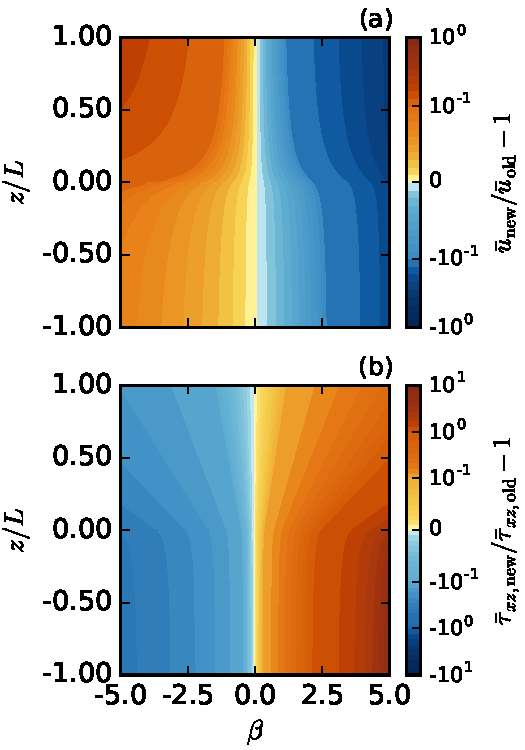
\includegraphics[width=2.4in]{figures/sample1}
\caption{A sample figure that is wrapped by text.}
\label{fig1}
\end{wrapfigure}

Lorem Khaled Ipsum is a major key to success. To be successful you've got to work hard, to make history, simple, you've got to make it. The first of the month is coming, we have to get money, we have no choice. It cost money to eat and they don't want you to eat. Fan luv. 

Surround yourself with angels, positive energy, beautiful people, beautiful souls, clean heart, angel. You smart, you loyal, you a genius. Give thanks to the most high. We the best. I told you all this before, when you have a swimming pool, do not use chlorine, use salt water, the healing, salt water is the healing.

In life there will be road blocks but we will over come it. The other day the grass was brown, now it's green because I ain't give up. Never surrender. You do know, you do know that they don't want you to have lunch. I'm keeping it real with you, so what you going do is have lunch. Don't ever play yourself. 

We don't see them, we will never see them. I'm up to something. Surround yourself with angels, positive energy, beautiful people, beautiful souls, clean heart.

\begin{wraptable}[15]{r}[0.01in]{4.5in}
\label{table1}
\caption{A sample table wrapped by text.}
\begin{center}
\vspace{-10pt}
\scriptsize
\begin{tabular}{  c  c  c  }
\hline
\hline
Stability & $M_u$ & $M_{\tau}$ \\ 
\hline\hline\\
Neutral & $\cfrac{z}{z_\Delta} - \cfrac{\ln(z/z_o)}{\ln(z_\Delta/z_o)}$ & $\cfrac{z}{z_\Delta} - \cfrac{1}{\ln(z_\Delta/z_o)}$\\\\
\hline \\
Stable & $\left(1 - \cfrac{\Psi}{2}\right)\cfrac{z}{z_\Delta} - \left(1 - \cfrac{\Psi_\Delta}{2}\right)
\left(\cfrac{\ln(z/z_o)-\Psi}{\ln(z_\Delta/z_o)- \Psi_\Delta}\right)$ & $\cfrac{z}{z_\Delta} - \cfrac{\left(1 - \cfrac{\Psi_\Delta}{2}\right)}{\ln(z_\Delta/z_o) - \Psi_\Delta}$\\\\
\hline \\
Unstable & $\cfrac{4}{3}\left[\left(\cfrac{1-x^3}{1-x_{\Delta}^{4}}\right) -  \left(\cfrac{1-x_{\Delta}^3}{1 - x_{\Delta}^{4}}\right)\left(\cfrac{\ln(z/z_o)-\Psi}{\ln(z_\Delta/z_o)- \Psi_\Delta}\right)\right]$ & $\cfrac{z}{z_\Delta} - \cfrac{\cfrac{4}{3}\left(\cfrac{1-x_{\Delta}^3}{1 - x_{\Delta}^{4}}\right)}{\ln(z_\Delta/z_o) - \Psi_\Delta}$\\\\
\hline
\hline
\end{tabular}
\end{center}
\end{wraptable}


Egg whites, turkey sausage, wheat toast, water. Of course they don't want us to eat our breakfast, so we are going to enjoy our breakfast. They don't want us to win. Major key, don't fall for the trap, stay focused.  It's the ones closest to you that want to see you fail. Always remember in the jungle there's a lot of they in there, after you overcome they, you will make it to paradise. The key to more success is to get a massage once a week, very important, major key, cloth talk.

% I found it useful to include a summary of the proposed work
% given in each subsection to help out reviewers.
\subsubsection{Specific tasks for this research component}
\begin{itemize}
\setlength\itemsep{0em}
\item Do a thing and blow your mind
\item Question your life choices
\item Drink coffee
\end{itemize}

\begin{center}
\begin{minipage}{.3\textwidth}
\begin{equation}
 \bar u = \bar u_{ll} + u_* \beta M_{u} \label{new_u}
\end{equation}
\end{minipage}
\begin{minipage}{.36\linewidth}
\begin{equation}
  \tau_{xz} = u_* u_{*ll} + \kappa u_*^2 \beta M_{\tau} \label{new_tau} \mbox{ ,}
\end{equation}
\end{minipage}
~\\Sample equations that consume minimal space.
\end{center}



%%%%%%%%%%%%%%%%%%%%%%%%%%%%%%
% Section 4: Management Plan %
%%%%%%%%%%%%%%%%%%%%%%%%%%%%%%
\section{Time Line and Management Plan}

\begin{table}[H]
\label{table1}
\renewcommand{\arraystretch}{0}
\caption{Project schedule.  PIs are Person One (P1), Person Two (P2), graduate student is GS, and the undergraduate student is US.\ Time frame gives the year each activity will occur.}
\scriptsize
\begin{tabularx}{\textwidth}{Y c c }
\hline
\hline
\textbf{Research Activity} & \textbf{Personnel} & \textbf{Time Frame}\\
\hline
Perform a task that sounds impressive & P2, US & Y1 \T\\
Perform another super-amazing task & P1, US & Y1 \T\\
Perform something else that may not be as sexy as the other things & P2, GS & Y1 \T\\
Wonder why you are such a terrible programmer & P1, US & Y1 \T\\
Analyze the results and stuff & P1, P2, SS & Y1,Y2 \T\\
Take the day off and grill some meat & P1, P2, SS & Y1,Y2 \T\\
Present findings at scientific meetings and publish results in peer-reviewed journals & P1, P2, US, GS & Y1, Y2, Y3\T\B\\
\hline
\hline
\end{tabularx}
\end{table}

%%%%%%%%%%%%%%%%%%%%%%%%%%%%%%
% Section 5: Science Merit   %
%%%%%%%%%%%%%%%%%%%%%%%%%%%%%%
\section{Scientific Merit}

You wanna know how I got these scars? My father was\ldots a drinker, and a fiend. And one night, he goes off crazier than usual. Mommy gets the kitchen knife to defend herself. He doesn't like that, not one bit. So, me watching he takes the knife to her, laughing while he does it. He turns to me and he says: ``Why so serious?''. He comes at me with the knife ``Why so serious?''. He sticks the blade in my mouth. ``Let's put a smile on that face.'' and\ldots Why so serious?

%%%%%%%%%%%%%%%%%%%%%%%%%%%%%%
% Section 6: Impact/Outreach %
%%%%%%%%%%%%%%%%%%%%%%%%%%%%%%

\section{Broader Impacts}
\label{broadimpacts}
\vspace*{-8pt}

This project will have direct impacts on research and education through access to simulation data products, student training, and K-12 outreach.  

\vspace{4pt}
\noindent \underline{\textit{Data Access}}: Maybe write about you will make data available.

\vspace{4pt}
\noindent \underline{\textit{Student Training}}: Write about how you will train students.

\vspace{4pt}
\noindent \underline{\textit{Some Other Outreach}}: Write about more outreach.

\vspace{4pt}
\noindent \underline{\textit{Dissemination}}: Write about how you will disseminate results (i.e., journal articles, workshops, etc).

%%%%%%%%%%%%%%%%%%%%%%%%%%%%%%
% Section 7: Prior NSF Work  %
%%%%%%%%%%%%%%%%%%%%%%%%%%%%%%
\section{Results from Prior Work}

\noindent \emph{\underline{Person One}}: No NSF support in the past five years \newline

\noindent The most relevant prior NSF award to the proposed project for \underline{Person Two} (Co-PI) is: (a) NSF PDM \#\#\#\#\#\#\#, \$000,000, MM/DD/YY to MM/DD/YY; (b) Title: Super Cool Project That Got Funded; (c) Accomplishments related to the {\bf intellectual merit} of this research project include something something. The {\bf broader impacts} include outreach at many levels. Something Something. To date, the grant has funded one post-doc and 1000 graduate students. The project has also involved 500 undergraduate students. (d) To date this project has resulted in 100 conference presentations, one million journal publications (cite them) with one under review (cite it) and two in preparation with well-developed drafts.

\nocite*
